\documentclass[tikz]{standalone}
\usepackage{tikz}
\usetikzlibrary{automata,positioning,arrows.meta}
\tikzset{
    >=Stealth,
    every edge/.style={draw,->,>=Stealth,thick},
    every loop/.style={draw,->,>=Stealth,thick}
}
\begin{document}

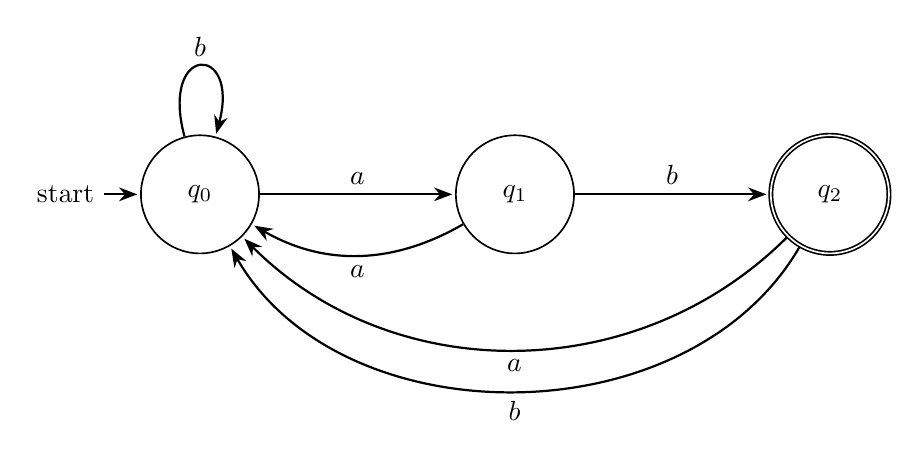
\begin{tikzpicture}[shorten >=1pt,auto,node distance=3cm,
                    semithick,
                    state/.style={circle,draw,minimum size=1.5cm}]

% States
\node[state,initial] (q1) at (0.00cm,0.00cm) {$q_0$};
\node[state] (q2) at (4.00cm,0.00cm) {$q_1$};
\node[state,accepting] (q3) at (8.00cm,0.00cm) {$q_2$};

% Transitions
\path (q1) edge [loop above] node {$b$} (q1);
\path (q1) edge node {$a$} (q2);
\path (q2) edge [bend left=30] node {$a$} (q1);
\path (q2) edge node {$b$} (q3);
\path (q3) edge [bend left=45] node {$a$} (q1);
\path (q3) edge [bend left=60] node {$b$} (q1);

\end{tikzpicture}
\end{document}
